\chapter{Introducción específica}

En este capítulo se presenta un resumen de los conceptos más relevantes acerca de la red TCN y su implementación en las formaciones de Trenes Argentinos, y se detallan las diferentes tecnologías utilizadas para el desarrollo del dispositivo de captura.

\section{La red TCN}

La red TCN es una combinación jerárquica de dos buses de datos para transmitir información dentro de una formación ferroviaria. El Multifunction Vehicle Bus (MVB) interconecta los diferentes dispositivos presentes dentro de cada vehículo, y el Wire Train Bus (WTB) interconecta los diferentes vehículos. Los componentes de la red TCN están estandarizados en la norma IEC 61375-1.

\begin{figure}[htbp]
	\centering
	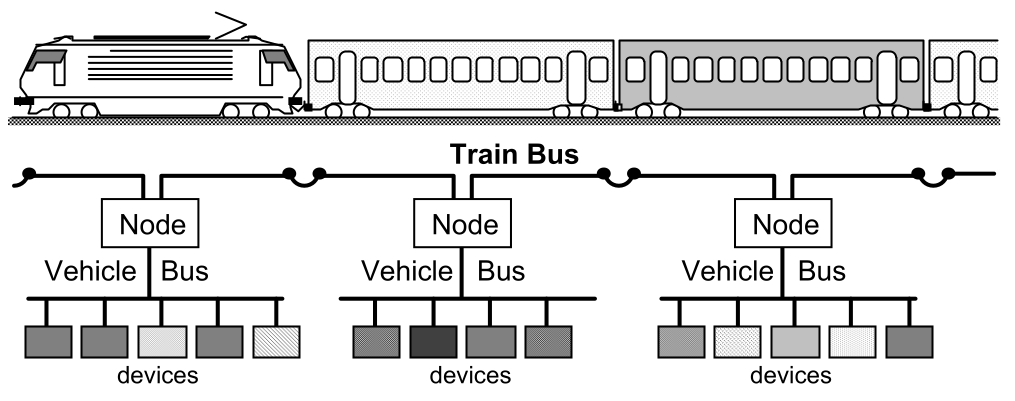
\includegraphics[width=.8\textwidth]{./Figures/tcn-mvb-wtb.png}
	\caption[Wire Train Bus y Multifunction Vehicle Bus]{Wire Train Bus y Multifunction Vehicle Bus.
        \\ \todo{CAMBIAR: La imagen original tiene copyright.}}
\end{figure}

Dado que el dispositivo desarrollado se conecta al bus MVB, a continuación se exponen las características principales de este bus de comunicación.

\subsection{El bus MVB}

El MVB es el bus que interconecta diferentes dispositivos ubicados en el mismo vehículo o en diferentes vehículos. Proporciona tanto la interconexión de equipos programables entre sí como la interconexión de estos equipos con sus sensores y actuadores. El MVB puede direccionar hasta 4095 dispositivos, y puede reemplazar a WTB en formaciones en las que los vehículos no son separados durante su operación normal.

El MVB transporta tres tipos de información:

\begin{itemize}
\item \texttt{Process\_Data}: transmisión \textit{broadcast} periódica con dirección de origen, con un período de hasta 1~ms.
\item \texttt{Message\_Data}: transmisión bajo demanda, con dirección de destino \textit{unicast} o \textit{broadcast}.
\item \texttt{Supervisory\_Data}: datos intercambiados con el propósito de resolución de eventos, transferencia de control \textit{master} o transmisión de información de tipo \texttt{Device\_Status}.
\end{itemize}

\subsection{Capa física MVB}

El bus MVB ofrece tres opciones para la capa física:

\begin{itemize}
\item El medio Electrical Short Distance (ESD), para distancias de hasta 20~m, que soporta hasta 32 dispositivos por segmento, con transceptores de tipo RS-485.
\item El medio Electrical Middle Distance (EMD), para distancias de hasta 200~m, que soporta hasta  32 dispositivos por segmento, con transformadores y transceptores compatibles con la norma IEC 61158-2 \cite{iec61158_2}.
\item El medio Optical Glass Fibre (OGF), para distancias de hasta 2000~m, y soporta conexiones punto a punto o subredes de topología tipo estrella.
\end{itemize}

En algunas formaciones el bus MVB puede abarcar varios vehículos, y un segmento EMD puede abarcar hasta 200~m, lo que equivale a unos 5 vehículos, sin repetidores. La norma recomienda este medio para conectar vehículos que se acoplan y desacoplan con frecuencia en la vía.

Las direcciones de los dispositivos se asignan durante la configuración de la red y no cambian durante la operación. Puede haber diferentes buses en un vehículo, interconectados mediante un \textit{gateway} al bus WTB.

\begin{figure}[htbp]
	\centering
	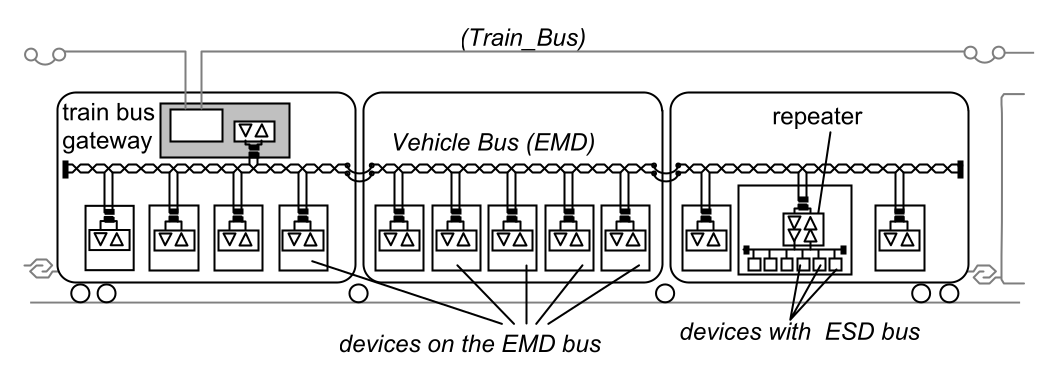
\includegraphics[width=1\textwidth]{./Figures/tcn-emd-esd-wtb.png}
	\caption[MVB abarcando tres vehículos]{MVB abarcando tres vehículos.
        \\ \todo{CAMBIAR: La imagen original tiene copyright.}}
\end{figure}

\subsection{Señalización MVB}

Todos los medios MVB operan a una velocidad unificada de 1,5~Mbit/s.
La información se transmite utilizando una codificación Manchester, que combina en una única señal la información y el \textit{clock}.
Un ``1'' se transmite como una transición negativa en el medio de una celda de bit, y un ``0'' se transmite como una transición positiva.

\begin{figure}[htbp]
	\centering
	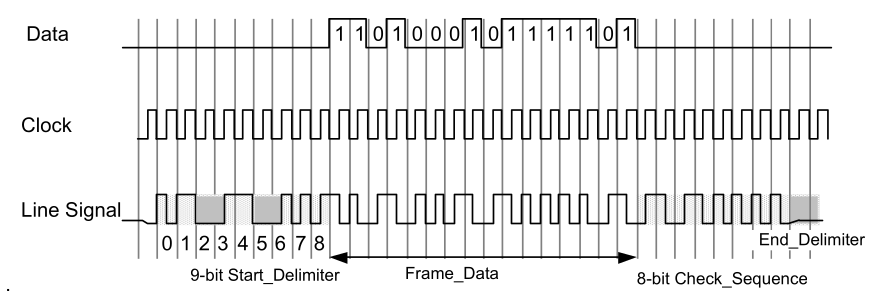
\includegraphics[width=1\textwidth]{./Figures/manchester.png}
	\caption[Delimitador de trama, información codificada con Manchester y la secuencia de verificación]{Delimitador de trama, información codificada con Manchester y la secuencia de verificación.
        \\ \todo{CAMBIAR: La imagen original tiene copyright.}}
\end{figure}

\subsection{Tramas MVB}

En el bus MVB se transmiten dos tipos de tramas:

\begin{itemize}
\item La trama \textit{master}, que es transmitida únicamente por el dispositivo maestro del bus.
\item La trama \textit{slave}, que es transmitida por un dispositivo esclavo en respuesta a una trama \textit{master}.
\end{itemize}

Ambos tipos de tramas son precedidas por un delimitador que marca el comienzo de la transmisión, y son sucedidas por una secuencia de verificación y un delimitador para marcar la finalización.

Una secuencia de una trama \textit{master} seguida de una trama \textit{slave} conforman un \textit{telegrama}.

\begin{figure}[htbp]
	\centering
	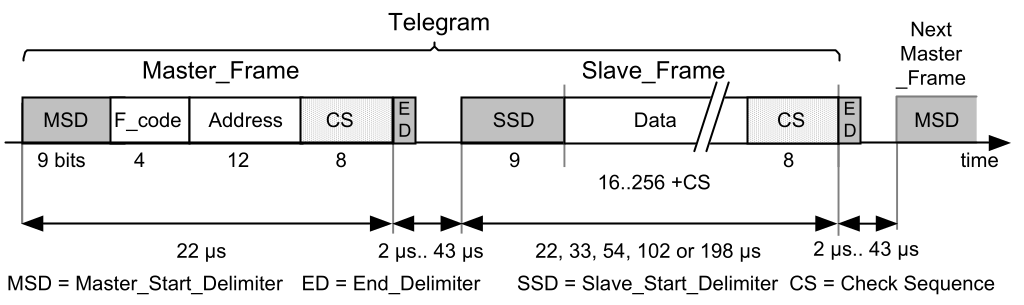
\includegraphics[width=1\textwidth]{./Figures/telegrama.png}
	\caption[Un telegrama MVB]{Un telegrama MVB.
        \\ \todo{CAMBIAR: La imagen original tiene copyright.}}
\end{figure}

Las tramas \textit{master} tienen una longitud fija de 16 bits (sin contar los delimitadores), e incluyen:

\begin{itemize}
\item Un código de 4 bits llamado \texttt{F\_code}, que indica el tipo y tamaño de la trama \textit{slave} esperada a continuación.
\item Un campo de 12 bits, que puede contener una dirección de destino, o parámetros específicos al \texttt{F\_code}.
\end{itemize}

Todos los dispositivos conectados al bus decodifican la trama \textit{master}. El dispositivo direccionado luego responde con su trama \textit{slave}, que a su vez puede ser recibida por otros dispositivos.

\section{TCN en Trenes Argentinos}

\section{Componentes del sistema}
